\documentclass[a4paper,12pt]{article}

% --- Pakete ---
\usepackage[utf8]{inputenc}   % Umlaute direkt eingeben
\usepackage[T1]{fontenc}
\usepackage[english]{babel}
\usepackage{lmodern}          % Schöne Schrift
\usepackage{geometry}         % Seitenränder anpassen
\usepackage{booktabs}         % Für schönere Tabellen
\usepackage{array}
\usepackage{setspace}         % Zeilenabstand
\usepackage{graphicx}
\usepackage{caption}
\usepackage{url}
\usepackage{todonotes}
\usepackage{float}
\usepackage{pgfplots}
\usepackage{xfp}      % provides \fpeval for calculations
\usepackage{multirow}

% --- Einstellungen ---
\geometry{a4paper, margin=2.5cm}
\setstretch{1.25}

% --- Dokument ---
\begin{document}
	
	% Titel
	\begin{center}
		{\LARGE \textbf{Praktikum Hochfrequenz-Schaltungstechnik WS25/26}} \\[1em]
		{\large  \textbf{Report}} \\[0.5em]
	\end{center}
	
	\begin{center}
		\begin{tabular}{|l|p{4cm}|l|p{4cm}|}
			\hline
			\textbf{Name:} &  Sebastian Grigorevski & \textbf{Matrikelnr.:} &  35690104 \\
			\hline
			\textbf{Versuchsnr.:} & 2 & \textbf{Datum:} & 01.12.2025 \\
			\hline
		\end{tabular}
	\end{center}
	
	\vspace{1cm}
	\setcounter{section}{1}  % setzt den Section Zähler auf 1
	\setcounter{subsection}{5}  % setzt den Subsection Zähler auf 5
	\setcounter{subsubsection}{0}  % setzt den Subsubsection Zähler auf 0
	
	\subsubsection{}
	
	The resistance $RQuelle$ and $RQuelle1$ of the transistor circuits  depict the internal resistance of the AC generator V2. It limits the current flowing towards the base of the transistor.
	Together with the capacitor it determines the high-pass characteristic of the coupling to the system.
	
	\subsubsection{}
	
	\begin{figure}[h]
		\centering
		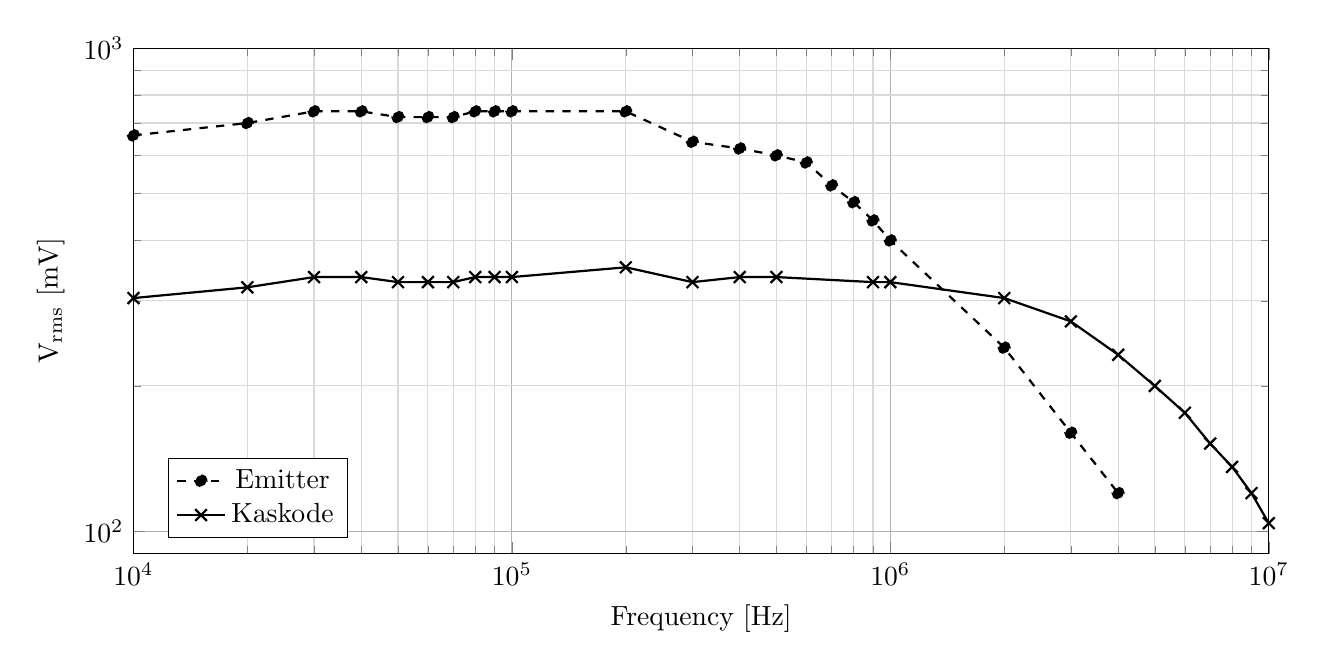
\begin{tikzpicture}
			\begin{axis}[
				width=16cm,
				height=8cm,
				xlabel={Frequency [Hz]},
				ylabel={V\textsubscript{rms} [mV]},
				xmode=log,
				log basis x={10},
				log basis y={10},
				ymode=log,
				grid=both,
				major grid style={gray!60},
				minor grid style={gray!30},
				mark size=2pt,
				legend pos=south west,
				xmin=1e4, xmax=1e7,
				ymin=90,  ymax=1e3,
				]
				
				% ---- First Trace ----
				\addplot[
				black,
				mark=*,
				thick,
				dashed
				] coordinates {
					(1e4, 660)
					(2e4, 700)
					(3e4, 740)
					(4e4, 740)
					(5e4, 720)
					(6e4, 720)
					(7e4, 720)
					(8e4, 740)
					(9e4, 740)
					(1e5, 740)
					(2e5, 740)
					(3e5, 640)
					(4e5, 620)
					(5e5, 600)
					(6e5, 580)
					(7e5, 520)
					(8e5, 480)
					(9e5, 440)
					(1e6, 400)
					(2e6, 240)
					(3e6, 160)
					(4e6, 120)
				};
				\addlegendentry{Emitter}
				
				% ---- Second Trace ----
				\addplot[
				black,
				mark=x,
				mark size=3pt,
				thick,
				] coordinates {
					(1e4, 304)
					(2e4, 320)
					(3e4, 336)
					(4e4, 336)
					(5e4, 328)
					(6e4, 328)
					(7e4, 328)
					(8e4, 336)
					(9e4, 336)
					(1e5, 336)
					(2e5, 352)
					(3e5, 328)
					(4e5, 336)
					(5e5, 336)
					(9e5, 328)
					(1e6, 328)
					(2e6, 304)
					(3e6, 272)
					(4e6, 232)
					(5e6, 200)
					(6e6, 176)
					(7e6, 152)
					(8e6, 136)
					(9e6, 120)
					(1e7, 104)
				};
				\addlegendentry{Kaskode}
				
			\end{axis}
		\end{tikzpicture}
		\caption{Frequency response of the root mean square voltage V\textsubscript{rms} of Emitter and Kaskode circuits}
		\label{fig: freqgang}
	\end{figure}
	
	\subsubsection{}
	
	Considering figure \ref{fig: amplif} the amplification at 10 mV lays at $\sim62$ for the emitter circuit and at $\sim30.4$ for the kaskode circuit. 
	Taking 89 \% of these amplification values results in $A_{\mathrm{emitter},0.89} = \fpeval{62*0.89}$ and $A_{\mathrm{kaskode},0.89} = \fpeval{30.4*0.89}$ for the different circuits. 
	Looking at the mentioned traces the calculated threshold for the emitter can be found at roughly below 100 mV where the data point is at a factor of 54. Moreover, for the kaskode $A_{\mathrm{kaskode},0.89}$ is reached at $\sim40$ mV (amplification of 27).
	This point of 0.89 of the amplification is can be translated to the decibel scale with $20 \cdot \log_{10}(0.89) \approx -1$ dB \cite{reinhold2023elektronische}.
	This point where the amplification decreases by one decibel is known as the \textit{compression}-point \cite{Strauss_GrundkursHF_3A}.
	
	\begin{figure}[h]
		\centering
		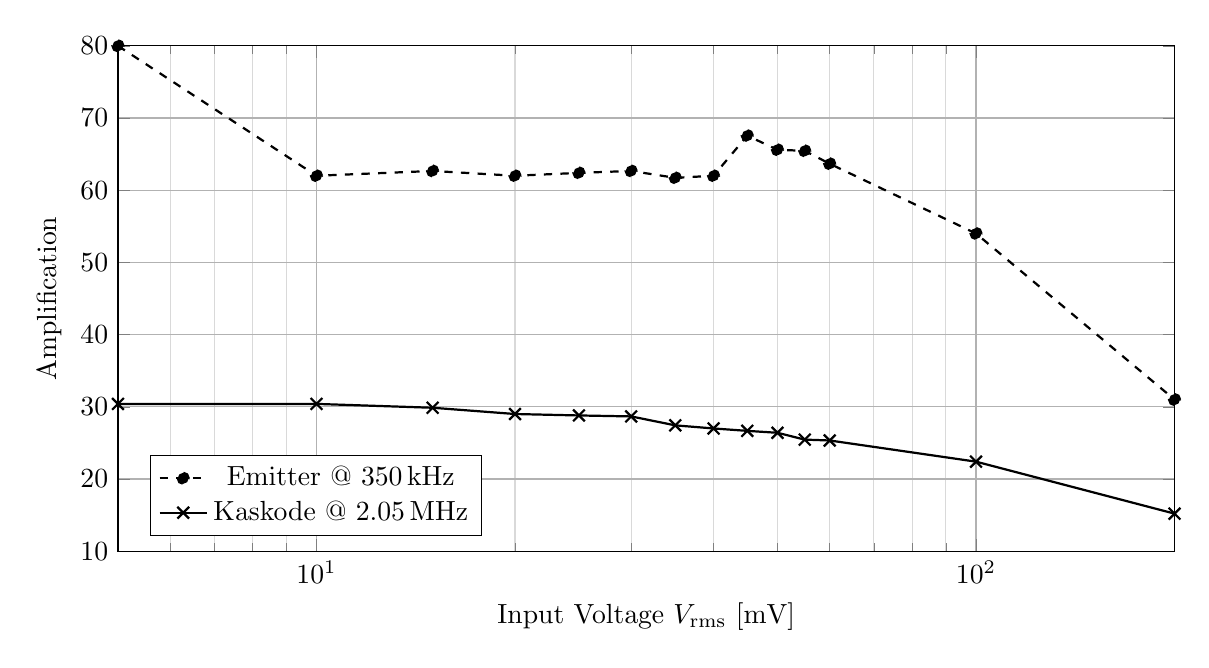
\begin{tikzpicture}
			\begin{axis}[
				width=15cm,
				height=8cm,
				xlabel={Input Voltage $V_{\mathrm{rms}}$ [mV]},
				ylabel={Amplification},
				grid=both,
				xmode=log,
				log basis x={10},
%				ymode=log,
%				log basis y={10},
%    			ytick={22.5, 25,27.5, 30, 32.5, 35, 37.5, 40},
				major grid style={gray!60},
				minor grid style={gray!30},
				mark size=2pt,
				legend pos=south west,
				xmin=5, xmax=200,
				ymin=10,  ymax=80,
				]
				
				% ==== 350 kHz Trace ====
				\addplot[
				black,
				mark=*,
				thick,
				dashed
				] coordinates { (5,400/5) (10,620/10) (15,940/15) (20,1240/20) (25,1560/25) (30,1880/30) (35,2160/35) (40,2480/40) (45,3040/45) (50,3280/50) (55,3600/55) 	(60,3820/60) (100,5400/100) (200,6200/200) };
%				] coordinates {
%					(5,  {20*log10(400/5)})
%					(10, {20*log10(620/10)})
%					(15, {20*log10(940/15)})
%					(20, {20*log10(1240/20)})
%					(25, {20*log10(1560/25)})
%					(30, {20*log10(1880/30)})
%					(35, {20*log10(2160/35)})
%					(40, {20*log10(2480/40)})
%					(45, {20*log10(3040/45)})
%					(50, {20*log10(3280/50)})
%					(55, {20*log10(3600/55)})
%					(60, {20*log10(3820/60)})
%					(100,{20*log10(5400/100)})
%					(200,{20*log10(6200/200)})
%				};
				\addlegendentry{Emitter @ 350\,kHz}
				
				% ==== 2.05 MHz Trace ====
				\addplot[
				black,
				mark=x,
				thick,
				mark size=3pt
				] coordinates { (5,152/5) (10,304/10) (15,448/15) (20,580/20) (25,720/25) (30,860/30) (35,960/35) (40,1080/40) (45,1200/45) (50,1320/50) (55,1400/55) (60,1520/60) (100,2240/100) (200,3040/200) };
%				] coordinates {
%					(5,   {20*log10(152/5)})
%					(10,  {20*log10(304/10)})
%					(15,  {20*log10(448/15)})
%					(20,  {20*log10(580/20)})
%					(25,  {20*log10(720/25)})
%					(30,  {20*log10(880/30)})
%					(35,  {20*log10(1080/35)})
%					(40,  {20*log10(1200/40)})
%					(45,  {20*log10(1320/45)})
%					(50,  {20*log10(1400/50)})
%					(55,  {20*log10(1400/55)})
%					(60,  {20*log10(1520/60)})
%					(100, {20*log10(2240/100)})
%					(200, {20*log10(3040/200)})
%				};
				\addlegendentry{Kaskode @ 2.05\,MHz}
				
			\end{axis}
		\end{tikzpicture}
		\caption{Amplification of the root mean square voltage V\textsubscript{rms} of Emitter and Kaskode circuits at their saturation frequencies.}
		\label{fig: amplif}
	\end{figure}

	\subsubsection{}
	
	The collector of the transistor of the emitter circuit bears a high impedance since it is directly connected to the system leading to a high AC voltages.
	On the other hand the collector Q1 is fed by the emitter of another transistor and sees a low impedance. This is because the base is connected to ground with the capacitor, thus the AC voltages are expected to be low.
	
	\subsubsection{}
	
	The transistor Q1 itself delivered an amplification of two measuring at $V_\mathrm{rms}=20\,$mV with an effective input voltage of 10 mV at 50 kHz.
	
	\subsubsection{}
	
	The Miller effect occurs from the transistors’ internal capacitances which introduce input–output feedback and reduce circuit gain. While this effect appears in a common-emitter stage, it is suppressed in a kascode. There, the base is effectively connected to ground through capacitor C2 together with resistors R1 and R2, diverting the AC signal so only a level potential exists at the emitter. Consequently, the feedback path is eliminated.
	
	\subsubsection{}
	
	The transit frequency of the given transistor is at $f_t = 250\,$MHz while a cutoff frequency was measured at $\sim700\,$kHz \cite{2N2222}. Their ratio can be calculated to $R_{t,c} = \frac{f_t}{f_{cutoff}} \approx 357.14$
	
	\subsubsection{}
	
	The transistor T2 of the circuit 103 of \cite{Elektor_303Circuits_1988} is being used in an base configuration since its base is directly connected to ground. This can be assumed since the capacitor is short circuited under high frequency. The same configuration can be seen with the transistor Q2. Meanwhile the transistor Q1 is set to be in emitter configuration for similar reason (and the name gives it away). Further the table below shows different characteristics of common configurations.
	
	\begin{table}[ht]
		\centering
		\caption{Comparison of basic transistor configurations taken from \cite{Gossner_GrundlagenDerElektronik_2011_8A}}
		\begin{tabular}{llccc}
			\toprule
			& Common-emitter & Common-collector & Common-base \\
			\midrule
			\multirow{1}{*}{input resistance $R_{\mathrm{in}}$ (AC)} & medium & large & small \\
	
			\multirow{1}{*}{output resistance $R_{\mathrm{out}}$ (AC)} & medium & small & medium \\
	
			\multirow{1}{*}{open-circuit voltage gain $V_{u0}$} & large & $\leq 1$ & large \\
	
			\multirow{1}{*}{current gain $V_{i}$} & medium / large & medium / large & $\leq 1$ \\
	
			\multirow{1}{*}{power gain $V_{p}$} & very large & medium / large & medium \\
	
			\bottomrule
		\end{tabular}
	\end{table}
	
	\subsubsection{}
	
	The oscilloscope probe was set to 1x and 10x for both the emitter circuit and kaskode circuit. For the emitter circuit no change in measurment of the cutoff frequency was observable. Measuring the kaskode circuit the cutoff frequency dropped by nearly half at 2.4 MHz with the 1x option compared with 4.1 MHz at 10x.
	This can be explained trough the absence of the Miller effect. In the kaskode circuit the bandwidth is determined by the output gate. There the increase of capacitance changing from 10x to 1x is significant and lowers the cutoff frequency. This cannot be observed in the emitter circuit since the Miller effect already determines a much lower cutoff frequency where the probe does not show aany difference.
	
	
	
	\vfill
	
	% --- Bibliography ---
	\bibliographystyle{plain}
	\bibliography{referenzen}
	
\end{document}